\subsection{Electromagnetic Calorimeter}\label{sec:cms_ecal}
The electromagnetic calorimeter (ECAL) is designed to reconstruct the energy of electromagnetic showers originating from electrons and photons for $\abs{\eta} < 3$. It is a homogenous calorimeter composed of scintillating crystals which emit light as a result of the charged particles created by electron and photon showers in the ECAL. By measuring the amount of light emitted, the energy of the particles can be inferred. 

Lead-tungstate (\pbw) was chosen to be the crystal material due to the following properties:
\begin{itemize}
  \item short radiation length: $X_0 = 0.89~\unit{cm}$, allowing for a compact calorimeter;
  \item narrow Moli\'ere radius: $R_M = 2.2~\unit{cm}$, resulting in a fine granularity;
  \item fast response time: 80\% of the scintillation light is emitted within 25~\unit{ns};
  \item good radiation hardness.
\end{itemize}
The ECAL is divided into two main components: the barrel (EB) and the endcaps (EE). The EB covers the region $\abs{\eta} < 1.479$, while the EE covers the region $1.479 < \abs{\eta} < 3.0$~\cite{CMS:2008xjf}. The overall structure of the ECAL is shown in \cref{fig:ecal}. 

\begin{figure}
  \centering
  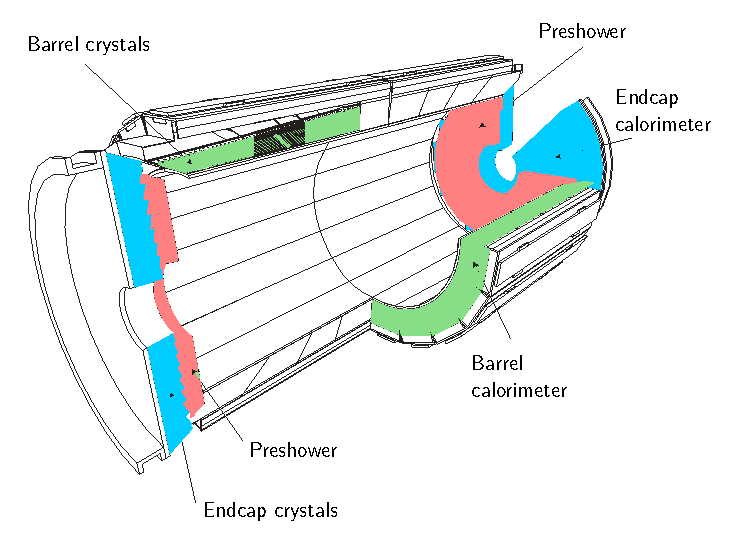
\includegraphics[width=\textwidth]{Figures/Detector/CMS/ecal_coloured.pdf}
  \caption[The CMS ECAL]{A schematic of the ECAL. Figure adapted from Ref.~\cite{CMS:2008xjf}.}\label{fig:ecal}
\end{figure}

The EB is composed of 61200 crystals, with a 360-fold granularity in $\phi$, and a 170-fold granularity in $\eta$. The crystals are tapered, with a front and rear cross-section of $22 \times 22~\unit{mm^2}$ and $26 \times 26~\unit{mm^2}$ respectively. The length of the crystals is 230~\unit{mm} (25.8$X_0$) and the front faces of the crystals are 1.3~\unit{m} from the beam line. To avoid particles from the IP aligning with cracks between crystals, the crystals are arranged in a quasi-projective geometry such that they point $3^{\circ}$ away from the vector that points towards the nominal IP. 

The EE is composed of 14648 crystals that are arranged 1.3~\unit{m} away from the nominal IP. The crystals have a front and rear cross-section of $28.6 \times 28.6~\unit{mm^2}$ and $30.0 \times 30.0~\unit{mm^2}$ respectively, with a length of 220~\unit{mm} (24.7$X_0$). Similar to the EB, the EE crystals are arranged in a quasi-projective geometry, and point towards a focus point 1.3~\unit{m} away from the nominal IP, pointing between $2^{\circ}$ and $8^{\circ}$ from the nominal IP. 

Additionally, a sampling calorimeter called the Preshower detector is placed in front of the endcap crystals. This detector has one layer of lead as an absorbing material, followed by two layers of orthogonally-placed silicon strip sensors of 1.9~\unit{mm} pitch. It provides a precise position measurement of incident electrons and photons which is particular useful for discriminating against photons originating from $\pi^0$ decays.

The Lead-tungstate (\pbw) crystals emit only 4.5 photoelectrons per \MeV, which is relativity low compared to other scintillating materials. To compensate for this, photomultipliers are used to amplify the signal. In the EB, silicon avalanche photodiodes (APDs) are used, with a gain of 50, and in the EE, vacuum phototriodes (VPTs) are used, with a gain of 10. The choice of the respective photomultipliers is due to the different configuration of the magnetic field and expected levels of radiation found in the barrel and endcaps~\cite{CMS:2008xjf}.

Finally, the intrinsic energy resolution of the ECAL is modelled by:
\begin{equation}
  \left(\frac{\sigma}{E}\right)^2 = \left(\frac{S}{\sqrt{E}}\right)^2 + \left(\frac{N}{E}\right)^2 + C^2,
\end{equation}
where $E$ is expressed in units of \GeV, and $S = 2.8\%$ is the stochastic term, $N = 12\%$ is the noise term, and $C = 0.3\%$ is the constant term, where the values are determined from test-beam data~\cite{CMS:2008xjf}. For photons with energy $E = \frac{1}{2}\mH \approx 62.5\GeV$, the energy resolution is approximately 0.3\GeV (0.5\%).